%(BEGIN_QUESTION)
% Copyright 2009, Tony R. Kuphaldt, released under the Creative Commons Attribution License (v 1.0)
% This means you may do almost anything with this work of mine, so long as you give me proper credit

Read and outline the introduction to the ``Energy in Chemical Reactions'' section as well as the ``Heats of Reaction and Activation Energy'' subsection of the ``Chemistry'' chapter in your {\it Lessons In Industrial Instrumentation} textbook.  Note the page numbers where important illustrations, photographs, equations, tables, and other relevant details are found.  Prepare to thoughtfully discuss with your instructor and classmates the concepts and examples explored in this reading.

\underbar{file i04109}
%(END_QUESTION)




%(BEGIN_ANSWER)


%(END_ANSWER)





%(BEGIN_NOTES)

Forcing atoms to separate from one another (i.e. breaking bonds) requires an investment of energy, which is represented as a positive $\Delta H$ value in a chemical equation.  This is an {\it endothermic} (energy-absorbing) reaction.

\vskip 10pt

Allowing atoms to form new bonds with one another releases energy, which is represented as a negative $\Delta H$ value in a chemical equation.  This is an {\it exothermic} (energy-releasing) reaction.  The lower the energy state of the bound molecule, the ``stronger'' those bonds are because much energy input is required to sever the bonds.

\vskip 10pt

Often, there is an initial investment of energy necessary to start a chemical reaction, even for exothermic reactions where there is a net release of energy.  This initial energy is called the {\it activation energy} for that reaction.  Catalyst materials work to minimize this activation energy, allowing all manner of chemical reactions to proceed more rapidly than they otherwise would.

$$\includegraphics[width=15.5cm]{i04109x01.eps}$$








\vskip 20pt \vbox{\hrule \hbox{\strut \vrule{} {\bf Suggestions for Socratic discussion} \vrule} \hrule}

\begin{itemize}
\item{} Explain the meaning of the $\Delta H$ written to the right of a chemical reaction.
\item{} Explain why a negative value of $\Delta H$ represents an {\it exothermic} reaction.
\item{} Explain why a positive value of $\Delta H$ represents an {\it endothermic} reaction.
\item{} Describe a practical example of {\it activation energy}.
\item{} Describe a practical example of a chemical reaction requiring little or no activation energy.
\item{} Explain why the exhaust system of an automobile contains a {\it catalytic converter}.
\item{} Explain why $\Delta H$ is unaffected by the presence or absence of a catalyst.  Hint: you may wish to appeal to the {\it Conservation of Energy} as an inviolable principle.
\item{} Explain why chemical equations do not contain the catalyst as either a reactant or a product.
\item{} A number of inventors have claimed to produce a device which connects to an automobile's engine and uses electricity from the engine's generator to split water into hydrogen and oxygen, which is then fed to the engine as fuel for it to run on.  The notion is that you may ``run your car on water'' instead of on a fuel such as gasoline.  Explain why this device cannot work, based on heats of reactions.
\end{itemize}













\vfil \eject

\noindent
{\bf Prep Quiz}

A general rule of chemical reactions is that:

\begin{itemize}
\item{} Forming chemical bonds releases energy
\vskip 5pt
\item{} Hydrogen refuses to bind with oxygen
\vskip 5pt
\item{} Breaking chemical bonds releases energy
\vskip 5pt
\item{} All exothermic reactions are spontaneous
\vskip 5pt
\item{} Forming chemical bonds absorbs energy
\vskip 5pt
\item{} Chemical bonds neither release nor absorb energy
\end{itemize}












\vfil \eject

\noindent
{\bf Prep Quiz}

An {\it endothermic} chemical reaction is one that:

\begin{itemize}
\item{} Happens spontaneously
\vskip 5pt
\item{} Generates light
\vskip 5pt
\item{} Increases in temperature
\vskip 5pt
\item{} Releases energy
\vskip 5pt
\item{} Results in larger molecules forming
\vskip 5pt
\item{} Absorbs energy
\end{itemize}



%INDEX% Reading assignment: Lessons In Industrial Instrumentation, Chemistry (energy in chemical reactions)

%(END_NOTES)


